% Digital Logic Report Template
% Created: 2020-01-10, John Miller

%==========================================================
%=========== Document Setup  ==============================

% Formatting defined by class file
\documentclass[11pt]{article}

% ---- Document formatting ----
\usepackage[margin=1in]{geometry}	% Narrower margins
\usepackage{booktabs}				% Nice formatting of tables
\usepackage{graphicx}				% Ability to include graphics

%\setlength\parindent{0pt}	% Do not indent first line of paragraphs 
\usepackage[parfill]{parskip}		% Line space b/w paragraphs
%	parfill option prevents last line of pgrph from being fully justified

% Parskip package adds too much space around titles, fix with this
\RequirePackage{titlesec}
\titlespacing\section{0pt}{8pt plus 4pt minus 2pt}{3pt plus 2pt minus 2pt}
\titlespacing\subsection{0pt}{4pt plus 4pt minus 2pt}{-2pt plus 2pt minus 2pt}
\titlespacing\subsubsection{0pt}{2pt plus 4pt minus 2pt}{-6pt plus 2pt minus 2pt}

% ---- Hyperlinks ----
\usepackage[colorlinks=true,urlcolor=blue]{hyperref}	% For URL's. Automatically links internal references.

% ---- Code listings ----
\usepackage{listings} 					% Nice code layout and inclusion
\usepackage[usenames,dvipsnames]{xcolor}	% Colors (needs to be defined before using colors)

% Define custom colors for listings
\definecolor{listinggray}{gray}{0.98}		% Listings background color
\definecolor{rulegray}{gray}{0.7}			% Listings rule/frame color

% Style for Verilog
\lstdefinestyle{Verilog}{
	language=Verilog,					% Verilog
	backgroundcolor=\color{listinggray},	% light gray background
	rulecolor=\color{blue}, 			% blue frame lines
	frame=tb,							% lines above & below
	linewidth=\columnwidth, 			% set line width
	basicstyle=\small\ttfamily,	% basic font style that is used for the code	
	breaklines=true, 					% allow breaking across columns/pages
	tabsize=3,							% set tab size
	commentstyle=\color{gray},	% comments in italic 
	stringstyle=\upshape,				% strings are printed in normal font
	showspaces=false,					% don't underscore spaces
}

% How to use: \Verilog[listing_options]{file}
\newcommand{\Verilog}[2][]{%
	\lstinputlisting[style=Verilog,#1]{#2}
}

\begin{document}

\title{ELC 2137 Lab 10: 7-segment Display with Time-Division Multiplexing}
\author{My Nguyen}

\maketitle

\section*{Summary}
This lab's purpose is to get a better understanding sequential circuit, develop a parameterized counter-timer module, and implement a 4-digit display using counter module. First part is to create a counter module that uses parameter to generate counter module with different number of bit for input and output. Then, create a wrapper module to test the counter module using different N parameters so the 4-digit display is smooth. Next, create show\_2c module, which which an 8-bit 2's complement and convert it to a sign bit. Afterward, create calc\_lab10 and import basys3.xdc with correct constraints as a top-level module to do on-board testing.

\section*{Simulation Waveform}
\begin{figure}[ht]
	\centering
	\includegraphics[width=\textwidth,trim=24cm 22.5cm 0.5cm 5.5cm,clip]{"counter"}
	\caption{Counter ERT}
	\includegraphics[width=\textwidth,trim=24cm 20cm 0.5cm 5.5cm,clip]{"show_2c"}
	\caption{show\_2c ERT}
\end{figure}


\section*{Code}
\Verilog[firstline=23,caption=Counter Implementation]{../verilog_code/counter.sv}
\Verilog[firstline=23,caption=Counter Test Bench]{../verilog_code/counter_test.sv}
\Verilog[firstline=23,caption=show\_2c Implementation]{../verilog_code/show_2c.sv}
\Verilog[firstline=23,caption=show\_2c Test Bench]{../verilog_code/show_2c_test.sv}
\Verilog[firstline=23,caption=Wrapper Implementation]{../verilog_code/wrapper.sv}
\Verilog[firstline=23,caption=Top-Level Implementation]{../verilog_code/calc_lab10.sv}


\section*{Pictures}
\begin{figure}[ht]
	\centering
	\includegraphics[width=12cm]{"board/4digit"}
	\caption{Displaying 4 digits with N = 20}
	\includegraphics[width=12cm]{"board/positive"}
	\caption{Adding hexadecimal 14 and 15 and outputing a decimal}
\end{figure}
\begin{figure}[ht]
	\centering
	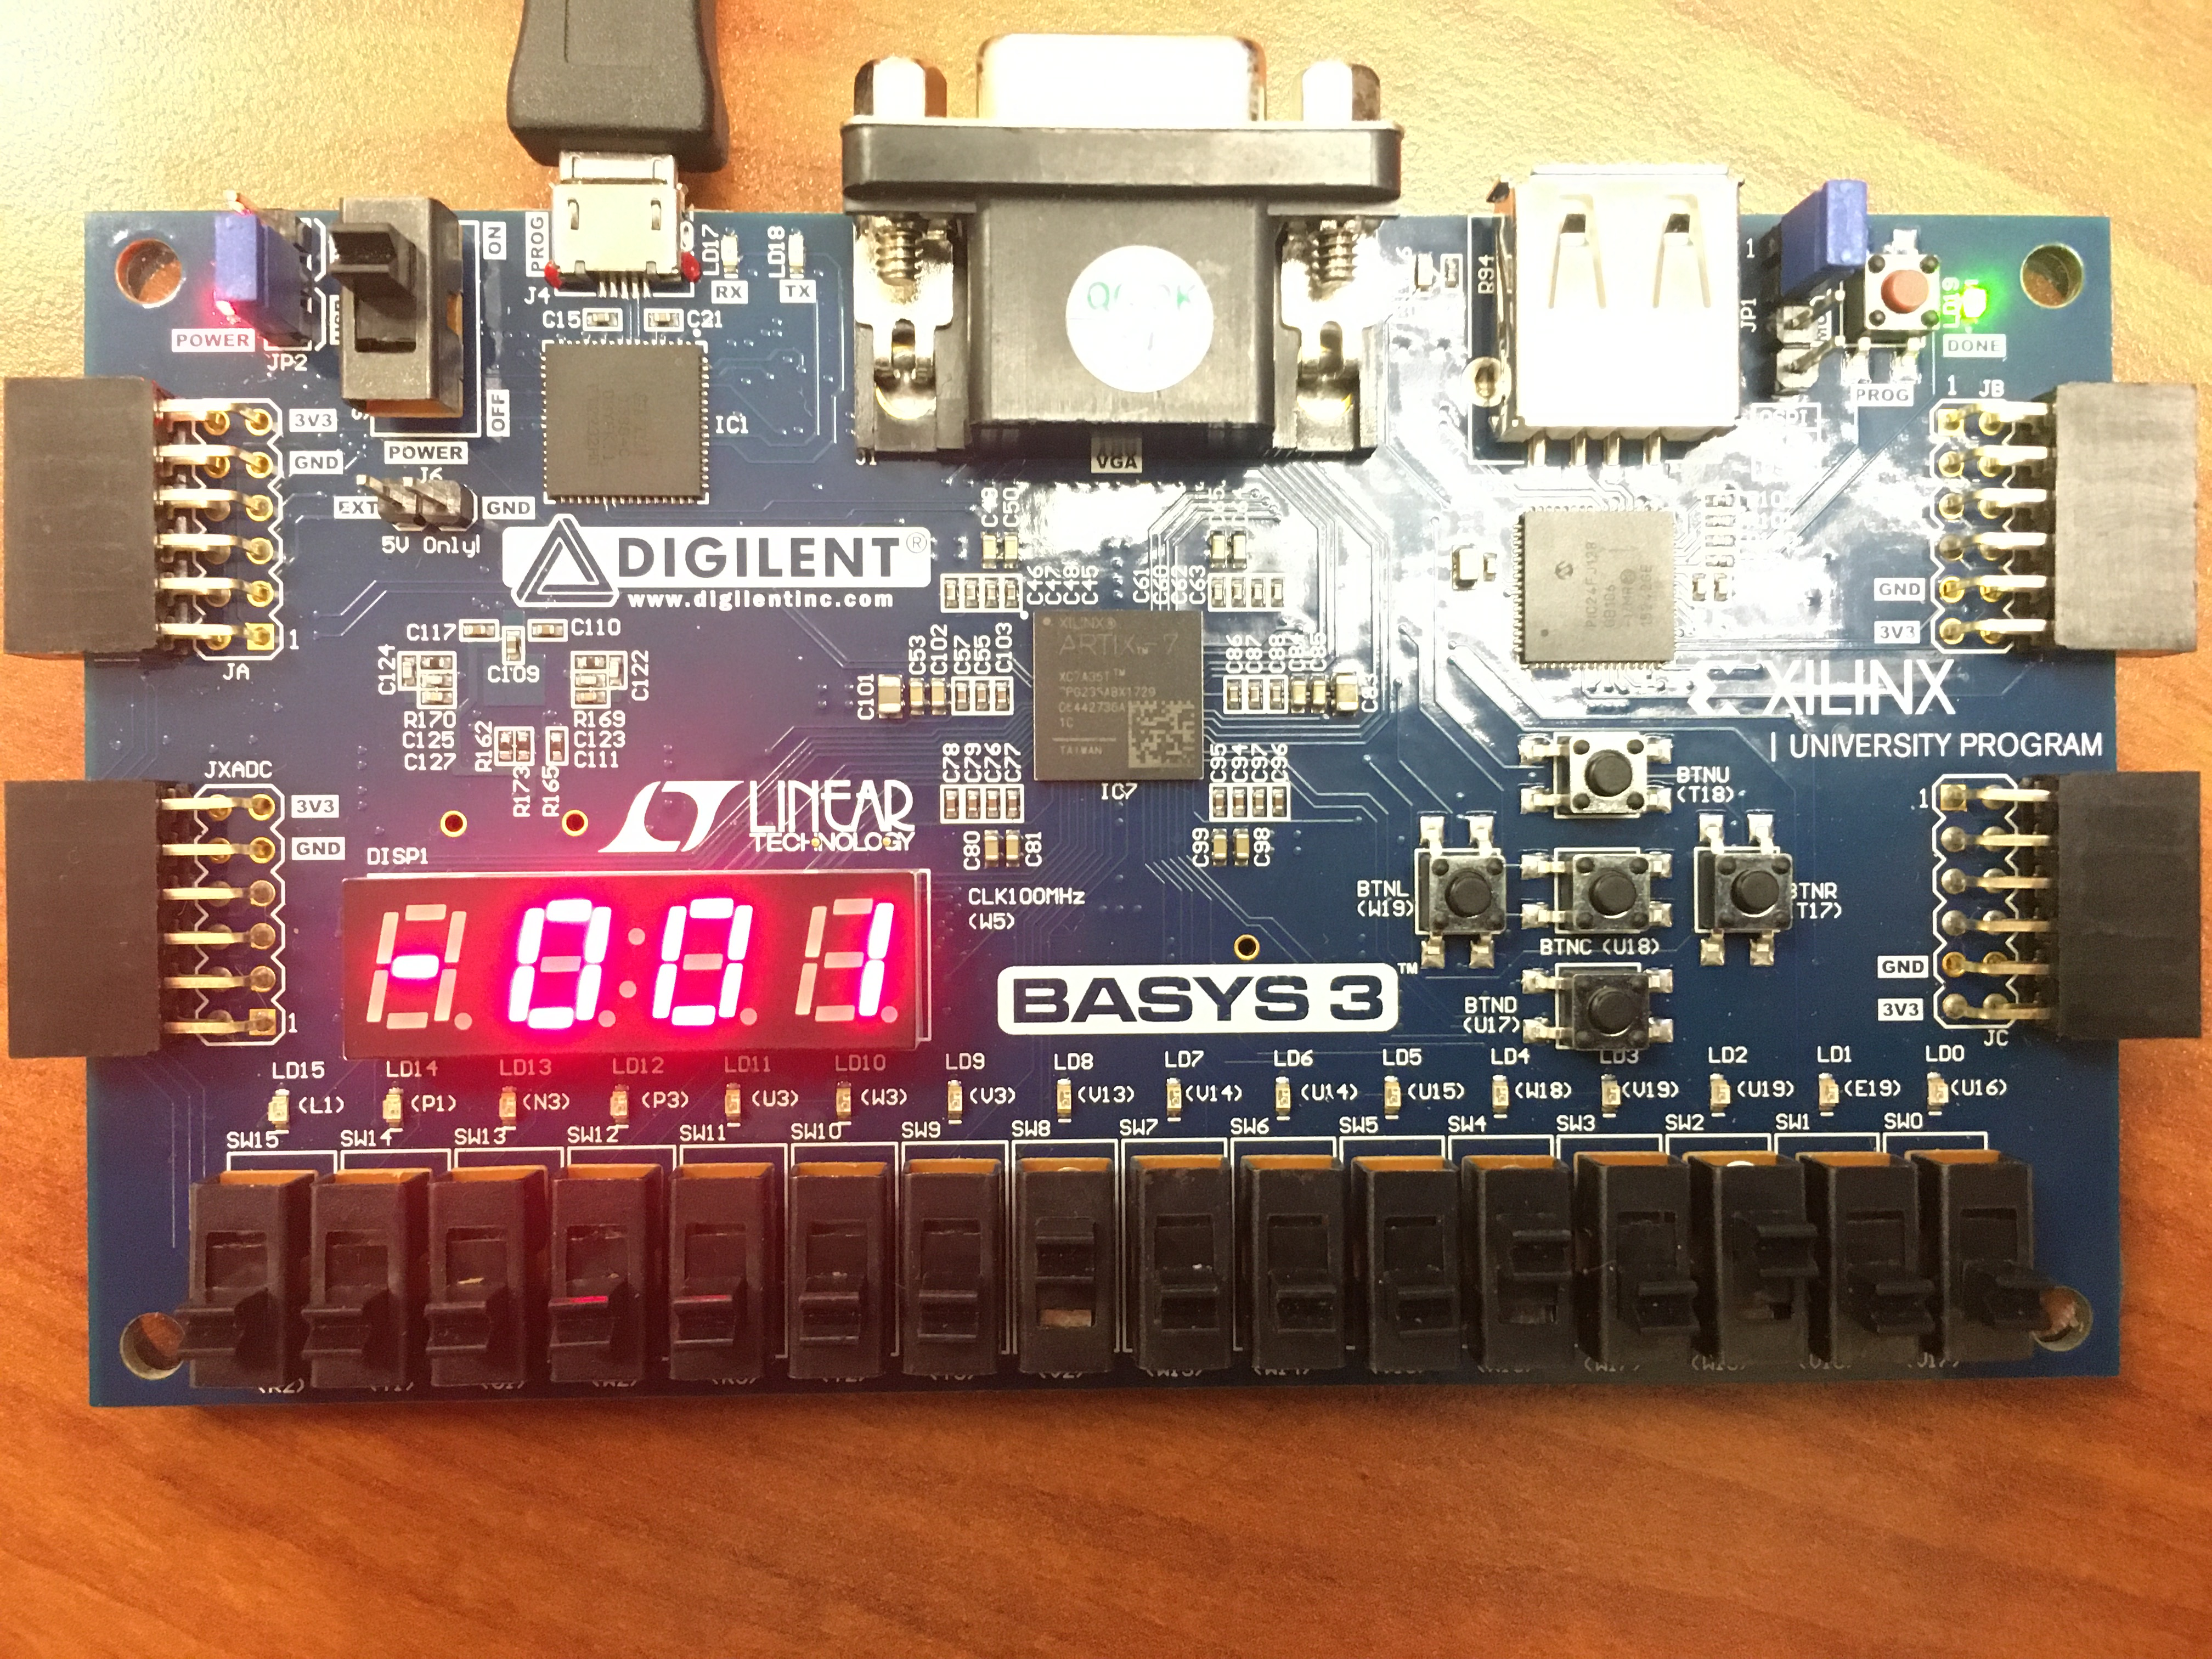
\includegraphics[width=12cm]{"board/negative}
	\caption{Subtracting hexadecimal 14 to 15 and outputing a decimal}
\end{figure}

\end{document}
